%%%
% Plantilla de Memoria
% Modificación de una plantilla de Latex de Nicolas Diaz para adaptarla 
% al castellano y a las necesidades de escribir informática y matemáticas.
%
% Editada por: Mario Román
%
% License:
% CC BY-NC-SA 3.0 (http://creativecommons.org/licenses/by-nc-sa/3.0/)
%%%

%%%%%%%%%%%%%%%%%%%%%%%%%%%%%%%%%%%%%%%%%
% Thin Sectioned Essay
% LaTeX Template
% Version 1.0 (3/8/13)
%
% This template has been downloaded from:
% http://www.LaTeXTemplates.com
%
% Original Author:
% Nicolas Diaz (nsdiaz@uc.cl) with extensive modifications by:
% Vel (vel@latextemplates.com)
%
% License:
% CC BY-NC-SA 3.0 (http://creativecommons.org/licenses/by-nc-sa/3.0/)
%
%%%%%%%%%%%%%%%%%%%%%%%%%%%%%%%%%%%%%%%%%

%----------------------------------------------------------------------------------------
%	PAQUETES Y CONFIGURACIÓN DEL DOCUMENTO
%----------------------------------------------------------------------------------------
%%% Configuración del papel.
% microtype: Tipografía.
% mathpazo: Usa la fuente Palatino.
\documentclass[a4paper, 11pt]{article}
\usepackage[protrusion=true,expansion=true]{microtype}
\usepackage{mathpazo}


% Indentación de párrafos para Palatino
\setlength{\parindent}{0pt}
  \parskip=8pt
\linespread{1.05} % Change line spacing here, Palatino benefits from a slight increase by default


%%% Castellano.
% noquoting: Permite uso de comillas no españolas.
% lcroman: Permite la enumeración con numerales romanos en minúscula.
% fontenc: Usa la fuente completa para que pueda copiarse correctamente del pdf.
\usepackage[spanish,es-noquoting,es-lcroman]{babel}
\usepackage[utf8]{inputenc}
\usepackage[T1]{fontenc}
\selectlanguage{spanish}


%%% Gráficos
\usepackage{graphicx} % Required for including pictures
\usepackage{wrapfig} % Allows in-line images
\usepackage[usenames,dvipsnames]{color} % Coloring code

%%% Matemáticas
\usepackage{amsmath}


%%% Bibliografía
\makeatletter
\renewcommand\@biblabel[1]{\textbf{#1.}} % Change the square brackets for each bibliography item from '[1]' to '1.'
\renewcommand{\@listI}{\itemsep=0pt} % Reduce the space between items in the itemize and enumerate environments and the bibliography
\usepackage{hyperref}
\hypersetup{
	colorlinks   = true,    % Colours links instead of ugly boxes
	urlcolor     = red,    % Colour for external hyperlinks
	linkcolor    = red,    % Colour of internal links
	citecolor    = blue      % Colour of citations
}
%%% CÓDIGO
\usepackage{listings}
\usepackage{courier}
\lstset{
	basicstyle=\footnotesize\ttfamily, % Standardschrift
	numbers=left,               % Ort der Zeilennummern
	numberstyle=\tiny,          % Stil der Zeilennummern
	stepnumber=1,               % Abstand zwischen den Zeilennummern
	numbersep=5pt,              % Abstand der Nummern zum Text
	tabsize=2,                  % Groesse von Tabs
	extendedchars=true,         %
	breaklines=true,            % Zeilen werden Umgebrochen
	keywordstyle=\color{red},
	frame=b,         
	%        keywordstyle=[1]\textbf,    % Stil der Keywords
	%        keywordstyle=[2]\textbf,    %
	%        keywordstyle=[3]\textbf,    %
	%        keywordstyle=[4]\textbf,   \sqrt{\sqrt{}} %
	stringstyle=\color{white}\ttfamily, % Farbe der String
	showspaces=false,           % Leerzeichen anzeigen ?
	showtabs=false,             % Tabs anzeigen ?
	xleftmargin=17pt,
	framexleftmargin=17pt,
	framexrightmargin=5pt,
	framexbottommargin=4pt,
	%backgroundcolor=\color{lightgray}
	showstringspaces=false      % Leerzeichen in Strings anzeigen ?        
	literate=
	{á}{{\'a}}1 {é}{{\'e}}1 {í}{{\'i}}1 {ó}{{\'o}}1 {ú}{{\'u}}1
	{Á}{{\'A}}1 {É}{{\'E}}1 {Í}{{\'I}}1 {Ó}{{\'O}}1 {Ú}{{\'U}}1
	{à}{{\`a}}1 {è}{{\`e}}1 {ì}{{\`i}}1 {ò}{{\`o}}1 {ù}{{\`u}}1
	{À}{{\`A}}1 {È}{{\'E}}1 {Ì}{{\`I}}1 {Ò}{{\`O}}1 {Ù}{{\`U}}1
	{ä}{{\"a}}1 {ë}{{\"e}}1 {ï}{{\"i}}1 {ö}{{\"o}}1 {ü}{{\"u}}1
	{Ä}{{\"A}}1 {Ë}{{\"E}}1 {Ï}{{\"I}}1 {Ö}{{\"O}}1 {Ü}{{\"U}}1
	{â}{{\^a}}1 {ê}{{\^e}}1 {î}{{\^i}}1 {ô}{{\^o}}1 {û}{{\^u}}1
	{Â}{{\^A}}1 {Ê}{{\^E}}1 {Î}{{\^I}}1 {Ô}{{\^O}}1 {Û}{{\^U}}1
	{œ}{{\oe}}1 {Œ}{{\OE}}1 {æ}{{\ae}}1 {Æ}{{\AE}}1 {ß}{{\ss}}1
	{ű}{{\H{u}}}1 {Ű}{{\H{U}}}1 {ő}{{\H{o}}}1 {Ő}{{\H{O}}}1
	{ç}{{\c c}}1 {Ç}{{\c C}}1 {ø}{{\o}}1 {å}{{\r a}}1 {Å}{{\r A}}1
	{€}{{\euro}}1 {£}{{\pounds}}1 {«}{{\guillemotleft}}1
	{»}{{\guillemotright}}1 {ñ}{{\~n}}1 {Ñ}{{\~N}}1 {¿}{{?`}}1   
}


\lstloadlanguages{% Check Dokumentation for further languages ...
	%[Visual]Basic
	%Pascal
	%C
	C++
	%%XML
	%%HTML
	%Java
}
%\DeclareCaptionFont{blue}{\color{blue}} 

%\captionsetup[lstlisting]{singlelinecheck=false, labelfont={blue}, textfont={blue}}
\usepackage{caption}
\DeclareCaptionFont{white}{\color{white}}
\DeclareCaptionFormat{listing}{\colorbox[cmyk]{0.43, 0.35, 0.35,0.01}{\parbox{\textwidth}{\hspace{15pt}#1#2#3}}}
\captionsetup[lstlisting]{format=listing,labelfont=white,textfont=white, singlelinecheck=false, margin=0pt, font={bf,footnotesize}
}

%% cosas 

\usepackage[margin=1in]{geometry}

\usepackage{times}

\usepackage{tikz}
\usetikzlibrary{arrows}
\usetikzlibrary{graphdrawing}
\usetikzlibrary{graphs}
\usegdlibrary{trees}

%----------------------------------------------------------------------------------------
%	DOCUMENTO
%----------------------------------------------------------------------------------------

\begin{document}
	
	
	\begin{titlepage}
		\begin{center}
			\vspace*{2cm}
			
			{\Huge \textbf Ejercicios de Algoritmica.}
			
			
			\vspace{0.5cm}
			
			
		    \centering 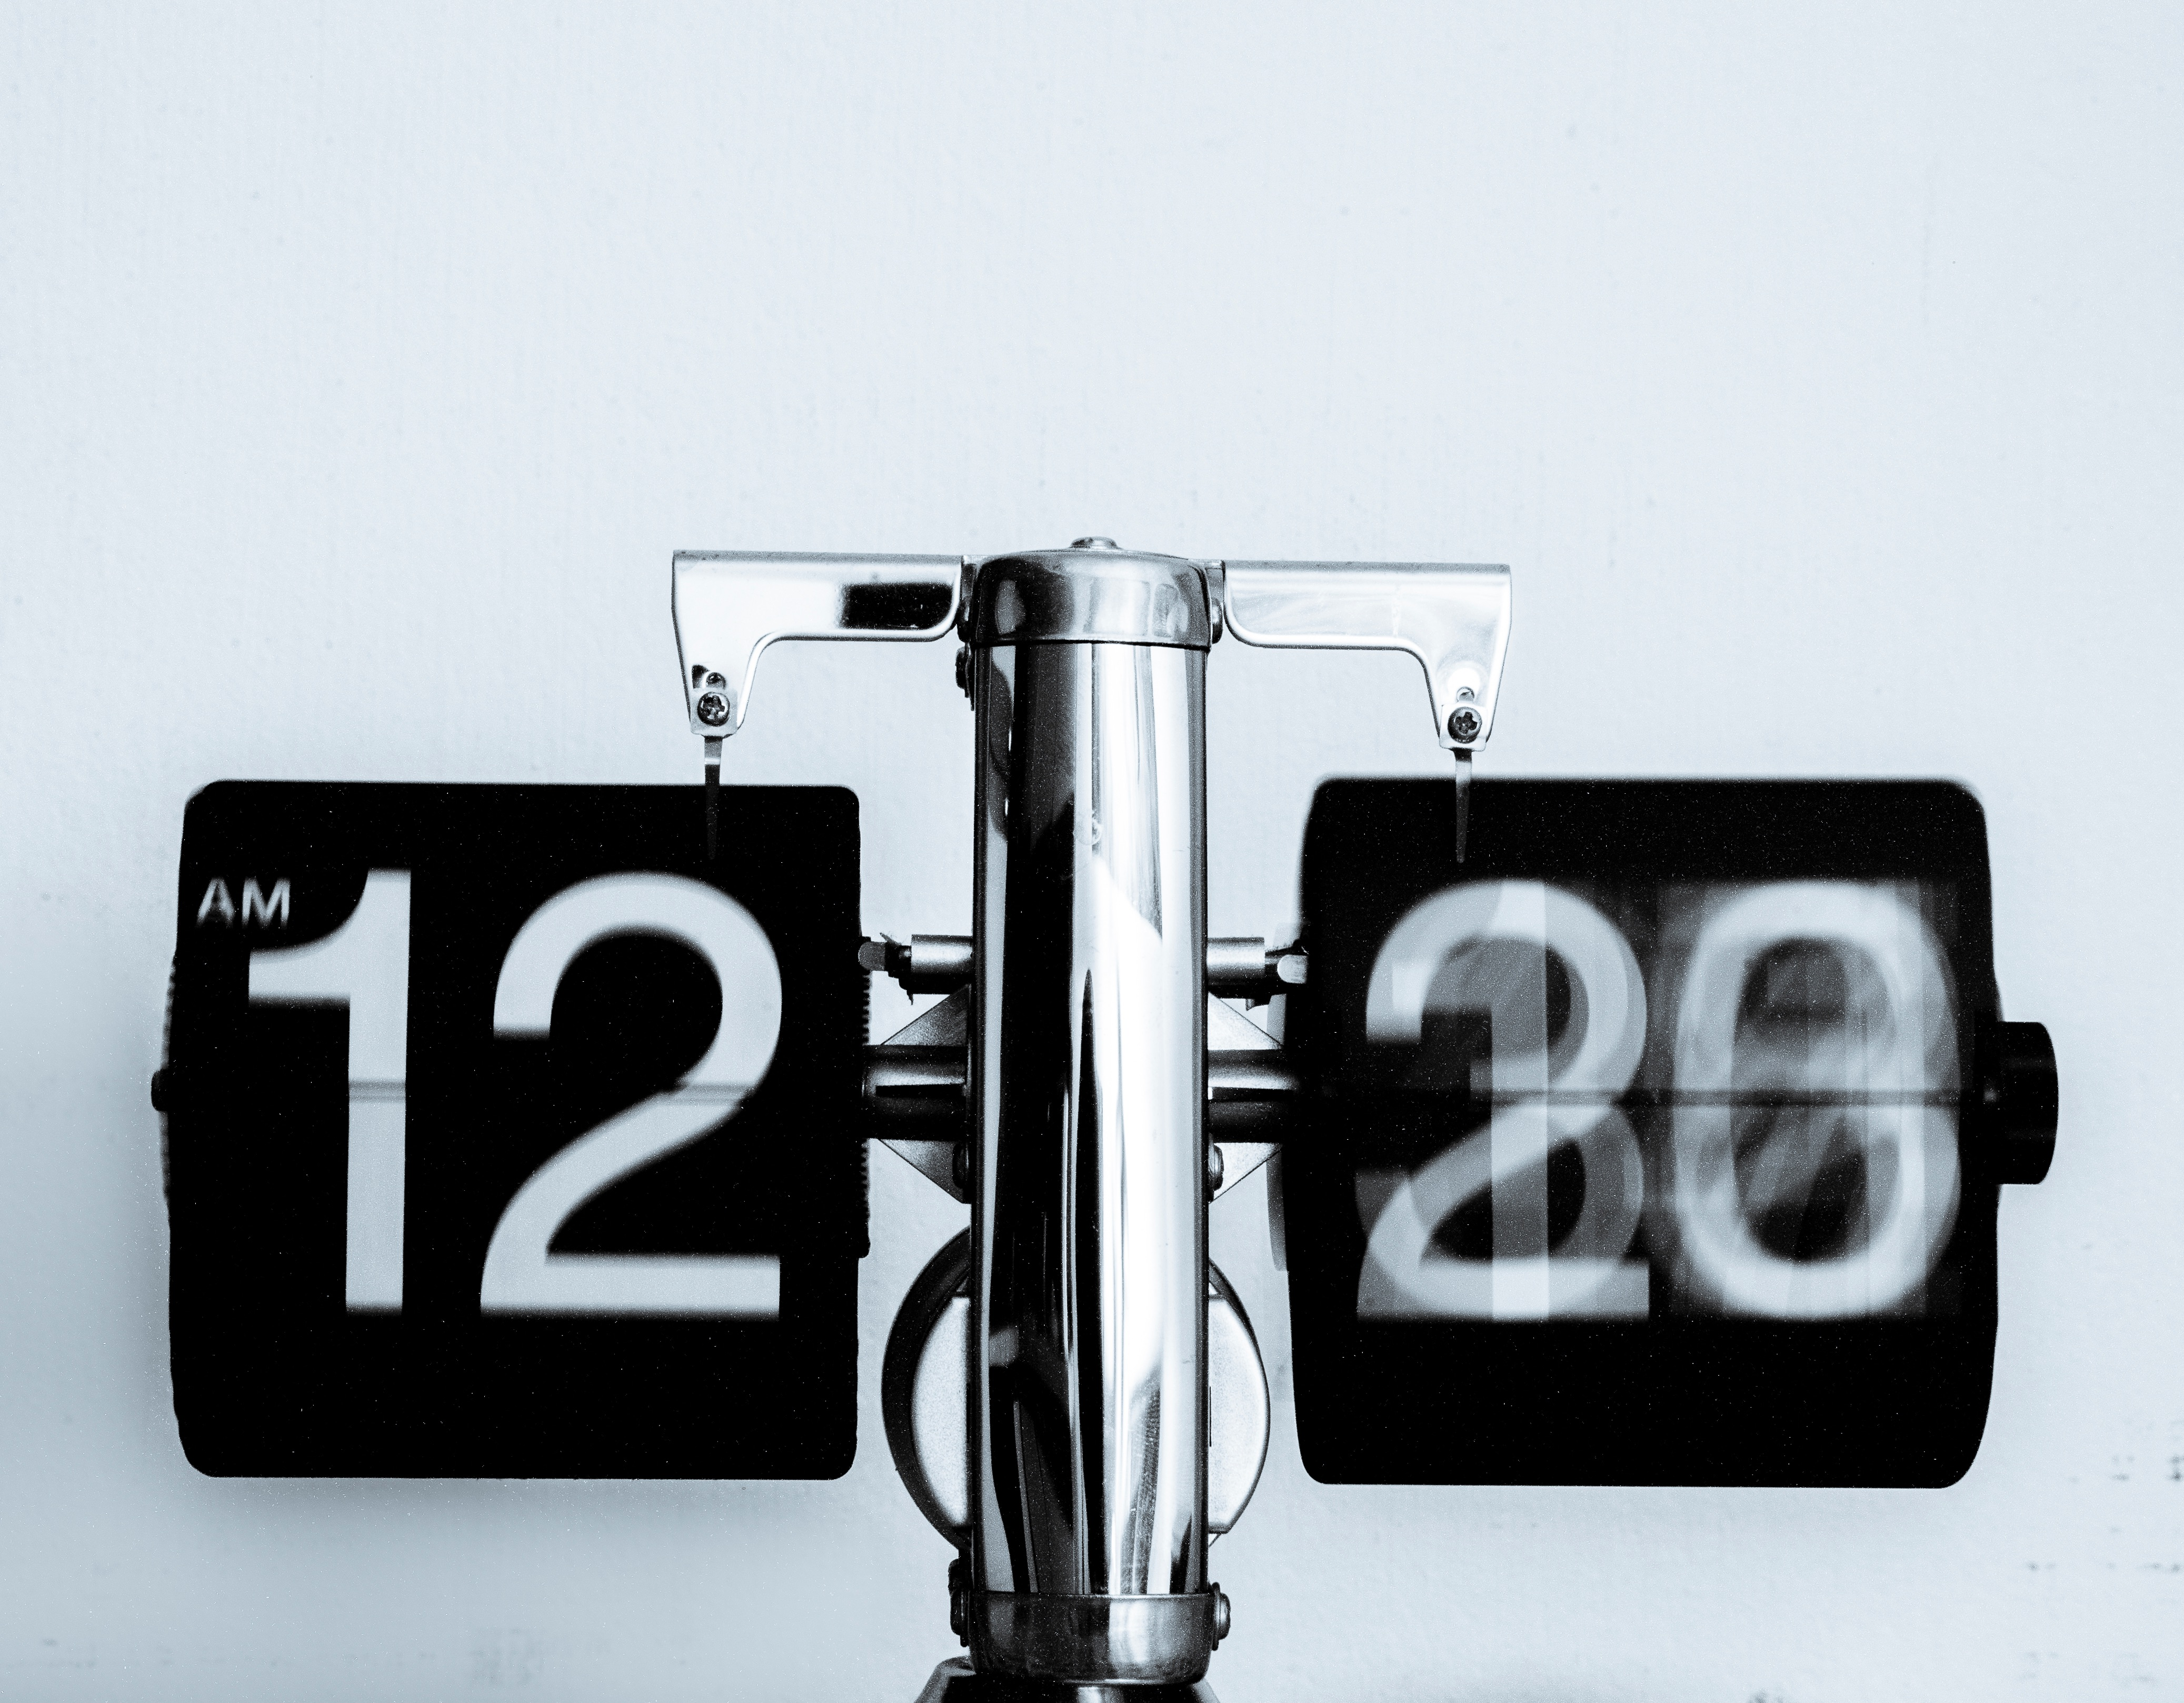
\includegraphics[width=0.9\textwidth]{cover.jpg}
		    
			
			\vspace{2cm}
			
			\textbf{Francisco Navarro Morales - GRG121 }
			
			\vfill
			
			Segundo curso del Grado de Ingeniería Informática\\
			Universidad de Granada\\
			curso 2016-2017\\
			
		\end{center}
	\end{titlepage}


%\maketitle % Print the title section

%% Resumen (Descomentar para usarlo)
\renewcommand{\abstractname}{Resumen} % Uncomment to change the name of the abstract to something else
%\begin{abstract}
% Resumen aquí
%\end{abstract}

%% Palabras clave
%\hspace*{3,6mm}\textit{Keywords:} lorem , ipsum , dolor , sit amet , lectus % Keywords
%\vspace{30pt} % Some vertical space between the abstract and first section


%% Índice
{\parskip=2pt
  \tableofcontents
}

%%% Inicio del documento

\pagebreak

\section{Búsqueda ternaria.}
?`Merece la pena implementar búsquedas ternarias? ?`Por qué se utilizan entonces las búsquedas binarias en vectores ordenados?

	\lstinputlisting[language=C++,label=BB,caption=Búsqueda binaria]{code/BinarySearch.cpp}
		\lstinputlisting[language=C++,label=BT,caption=Búsqueda ternaria]{code/TernarySearch.cpp}
		
		Considerando que la parte ligada a la división y combinación de problemas es igual al número de comparaciones que requiere cada algoritmo, tenemos que:
		
		Para la búsqueda binaria: $t(n)=t(n/2)+2$ en el peor caso.
		Para la búsqueda ternaria: $t(n)=t(n/3)+4$ en el peor caso.
		
		Entonces, sea $a$ el número de combinaciones necesario para cada caso, y $b$ el número de partes en que se divide el problema en cada caso, sea: $n=b^k$ tenemos:
		
		$$t(n)=t(b^k)=t(b^{k-1}+a)\rightarrow t_k - t_{k-1} = a$$
		
 Tenemos entonces una recurrencia lineal no homogénea, cuya parte homogénea tiene la raíz $x-1$ y cuya parte no homogénea también tiene la raíz $x-1$, luego:
		
		$$t_k = c_1\times 1^{k} + c_2\times k \times 1^k = c_1 + c_2 \times k$$
		
		Como $k=log_bn$ tenemos que $t(n) = c_1 + c_2 \times log_bn$ 
		
		En el caso de la búsqueda binaria: $t(n) = c_1 + c_2 \times log_2n$ y en el caso de la búsqueda ternaria: $t(n) = c_1 + c_2 \times log_3n$ 
		
		Si hallamos los coeficientes nos queda:
		
		\textbf{Búsqueda binaria:}
		
		$t(1)=1$ y $t(2)=3$ entonces, como $t(1)=c_1+log_21=c_1+0=1$, $c_1=1$. Entonces $t(2)=1+c_2\times log_22 = c_2+1 = 3\rightarrow c_2 = 2$
		
		luego $t(n) = 2log_2n + 1$
		
		\textbf{Búsqueda ternaria:}
		
		$t(1)=1$ y $t(3)=5$ entonces, $t(1)=c_1+log_31=c_1+0=1$, $c_1=1$. Entonces $t(3)=1+c_2 \times log_33 = c_2+1 = 5 \rightarrow c_2 = 4$ 
		
		luego $t(n) = 4log_3n + 1$
		
		Haciendo un cambio de base sabemos que $log_3n=\frac{log_2n}{log_23}$ luego, despreciando la parte constante, y comparando los dos tiempos tendríamos:
		
		$$\frac{2log_2n}{4log_3n}=\frac{log_2n \times log_23}{2 \times log_2n}=\frac{log_23}{2}<1$$
		
		(Ya que $log_23$ es menor que dos porque $2^2=4>3$) luego la ejecución de la búsqueda binaria es más rápida que la búsqueda ternaria (utilizarla en lugar de la búsqueda ternaria proporciona una ganancia de 1.261859507)
		
\section{Cuadrado latino.}	
Un cuadrado latino es un tablero de n x n posiciones, cada una de las cuales posee un
color escogido entre n colores diferentes. Ha de cumplir la restricción de que no puede haber
colores repetidos en ninguna de sus filas ni en ninguna de sus columnas. Diseñar un algoritmo que imprima todos los posibles cuadrados latinos de tamaño n x n.

Podemos tratar de resolver este problema con el paradigma de Backtracking, ya que se puede implementar buscando todas las combinaciones posibles paso a paso (para dejar de buscar en las combinaciones que contienen elementos que ya hemos comprobado que no son válidos) y no sería sencillo implementar un criterio de `valores' para los nodos, por lo que utilizar Branch\&Bound no sería posible, en principio.

Respecto al modo de codificar la solución y de representar el árbol de búsqueda, he optado por representar cada posición del vector que representaría internamente la matriz cuadrada que representa al cuadrado latino como un nivel del árbol de búsqueda. Así, no será necesario almacenar la solución como tal, sino que bastaría con almacenar, para cada nodo, su predecesor, y al llegar a un nodo terminal podríamos extraer la solución recuperando uno a uno sus antecesores hasta llegar al comienzo.

Así, por ejemplo, para el tamaño $3\times 3$, el árbol de búsqueda sería (en los primeros niveles) tal que:

\begin{tikzpicture}[>=stealth, every node/.style={circle, draw, minimum size=0.75cm}]
\graph [tree layout, grow=down, fresh nodes, level distance=0.5in, sibling distance=0.5in]
{
	x -> { 
		1 -> { 2 -> { 3 -> { 2 -> { 3 -> {1 }},3 } }, 3 -> { 2 -> { 2, 3 } }},
		2 -> { 1 -> { 3 -> { 1,3 } }, 3 -> { 1-> { 1,3 } }},
		3 -> { 1 -> { 2 -> { 1,2 } }, 2 -> { 1 -> { 1,2 } }}
	} 
};
\end{tikzpicture}

Es un árbol permutacional en los tres primeros niveles, porque la primera fila puede contener todas las permutaciones posibles de $n$ valores.
A partir del  tercer nivel, como se ve en el camino de la izquierda, las restricciones impuestas por la fila anterior (rellenada en los 3 niveles anteriores) hacen que los valores posibles para cada posición sean menos y la anchura de la búsqueda queda reducida.

Aún así, podremos afirmar que la profundidad de la búsqueda será de $n^2$ niveles. Por otro lado, la ventaja de utilizar este método es que podremos encontrar todas las posibilidades y no necesitaremos almacenar una matriz por cada nodo, sino que podremos `construir' la matriz al llegar a un nodo hoja para imprimir la solución correspondiente al mismo. Además, determinar que un nodo es terminal (hoja) es tan simple como comprobar que su profundidad sea $n^2$.

Así, utilizando, por ejemplo, una estructura map en la que la clave sea una posición del vector y el valor sea el color asignado, el esquema del algoritmo sería:

(se llamaría a la función con nivel= 1 la primera vez)

Colorea(nivel, n):
\begin{itemize}
	\item Si nivel == n*n
	\begin{itemize}
		\item AlmacenaResultado()
	\end{itemize}
	\item Si no:
	\begin{itemize}
		\item siguiente\_color = 0
		\item repetir mientras siguiente\_color < n
		\begin{itemize}
			\item si EsValido(siguiente\_color, nivel) // función criterio.
			\begin{itemize}
				\item color[nivel] = siguiente\_color
				\item Colorea(nivel+1,n)
			\end{itemize}
		\end{itemize}
	\end{itemize}
\end{itemize}

Cuando se encuentre un camino en el que no es posible añadir ningún valor a la matriz, al salir del bucle marcado por siguiente\_color se romperá la recursividad y el algoritmo seguirá buscando por el siguiente color posible del nodo anterior (aquí es donde se da el backtracking). En los caminos en los que siempre se pueda añadir un valor de los $n$ posibles, al llegar al nivel $n*n$ se Almacenará la solución y se romperá la recursividad, de forma que se sigan haciendo todas las comprobaciones posibles, por lo que finalmente se encuentran todas las soluciones.

AlmacenarResultado() será una función que almacena en una matriz o vector los valores que devuelve el mapa color para cada valor desde $1$ hasta $n$, que serán los colores que corresponden al cuadro latino.

EsValido será una función que comprueba si hay alguna restricción para colocar el color $siguiente\_color$ en el nivel dado. Funcionaría calculando en primer lugar la fila a la que corresponde el nivel: fila = nivel\\n y la columna en la que está: columna = nivel\%n. A continuación comprobaría si los elementos previos de la misma fila tienen el mismo valor (en tal caso devuelve false), es decir, si color[k] con k tomando los valores desde fila*(n-1)+1 hasta fila*(n-1)+columna-1. En segundo lugar comprobaría (si no se hubiera dado ningún conflicto en la fila) si hay algún elemento en la misma columna, en una fila anterior, con el mismo color. Es decir, si colores[k] es igual a siguiente\_color con k tomando valores: fila*(i)+columna con i <= fila-1 empezando en 0. 

\section{Horario de partidos}
IV.5. Se ha de organizar el horario de un campeonato entre n jugadores. Cada uno ha de
jugar exactamente una vez contra cada adversario. Además, cada jugador ha de jugar
exactamente un partido diario. Suponiendo que n es potencia de 2, diseñar e implementar un
algoritmo que construya el horario y permita terminar el campeonato en n-1 días. Indicar el
esquema utilizado. Analizar el coste del algoritmo.

Se puede resolver utilizando una matriz $N\times N$ (en realidad no hace falta rellenar toda la matriz, porque la solución final será una matriz simétrica pero lo podemos implementar rellenando la matriz entera para mayor comodidad a la hora de programar y entender el código).

La idea es que a cada jugador $i$ le corresponden la fila y la columna $i$. (Llamaremos a los jugadores A,B,C... pero a cada uno le corresponde el número que representa su fila y su columna). Entonces, el contenido de la posición $[i][j]$ será el día en que tendrá lugar el partido entre los jugadores $i$ y $j$. Como un jugador no jugará consigo mismo, las posiciones en las que $i==j$ tomarán el valor $-1$.

En principio podría parecer un algoritmo suficientemente sencillo como para utilizar un enfoque Greedy para resolverlo, pero dado que no podemos asegurar que en todo momento va a haber un valor posible para una posición de la tabla de horarios (Puede darse el caso de que las posiciones previas a una dada en su fila y en su columna contengan todos los valores posibles desde 1 hasta $n-1$), necesitamos implementar un algoritmo que permita rectificar decisiones incorrectas. Necesitamos un esquema de Backtracking.

Los niveles del árbol de búsqueda se corresponderán con la asignación de un valor a la posición $M[i][j]$ con $j>i$ donde $M$ representa la que será la matriz solución (tabla de encuentros en la que cada valor representa el día en que se enfrentan los jugadores $i$ y $j$).

Utilizaré un esquema recursivo para definir la solución del problema:
\pagebreak
AsignaFecha(jugador1,jugador2,njugadores)
\begin{itemize}
	\item dia = 1
	\item para cada valor $M[a][b]$ donde a y b toman valores iguales o menores que la fila/columna que representa a cada jugador, probando todas las combinaciones, si las hay: 
	\begin{itemize}
		\item Si dia < n, entonces: 
			\begin{itemize}
			\item si $M[a][b]==dia$, entonces dia = dia + 1 y vuelve al primer par $a,b$.
			\item si no, $M[jugador1][juador2] = dia $ y:
				\begin{itemize}
				\item dia = dia +1. a y b vuelve a ser el primer par posible.
				\item Si jugador2 == n-1 y jugador1 < n-1, entonces AsignaFecha(jugador1+1,jugador2,njugadores)
				\item Si no, si jugador2 < n-1, entonces AsignarFecha(jugador1,jugador2+1)
				\item Si no, entonces ha encontrado la solución, la almacena o la muestra por pantalla.
				\end{itemize}
			\end{itemize}	
		\item Si no, termina la función y se rompe la recursividad.
	\end{itemize}
\end{itemize}

La primera vez se llamará al algoritmo con: AsignaFecha(0,1,njugadores)

Los casos en los que no se puede añadir ningún valor a una posición se resuelven con el bucle de `si dia < n' porque cuando se prueban todos los días terminará la función y se romperá la recursividad. Como antes de llamar a la función recursivamente se ha hecho dia = dia + 1, si siguen quedando días válidos sin probar, se seguirán probando, y si no, se volverá a romper la recursividad tantas veces como sea necesario.


\section{Aplicar el algoritmo de Dijkstra al siguiente grafo:}
 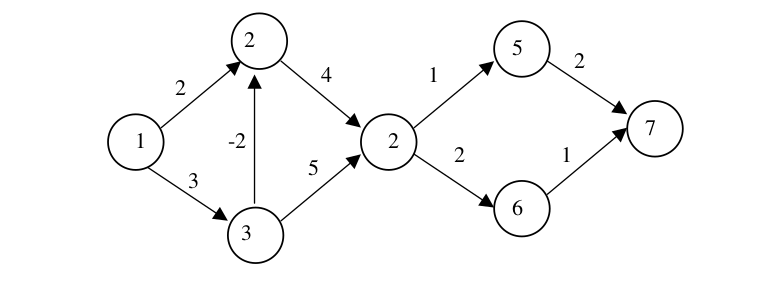
\includegraphics[width=0.9\textwidth]{grafo.png}
 *nota hay dos nodos marcados como 2, el de la derecha se considera un 4.
 
Uno de los requisitos para que algoritmo de Dijkstra encuentre un camino óptimo es que los costes de las aristas sean todos positivos. No obstante, se puede seguir aplicando el algoritmo a este nodo aunque posiblemente no devuelva el camino óptimo. 

Almacenamos una lista de nodos abiertos, considerando el nodo 1 el origen. Para cada nodo almacenamos el coste de llegar a él desde 1 y el nodo desde el que se llega con mejor coste. El algoritmo funciona de la siguiente forma: 

* Abrimos el nodo 1 con coste 0 y padre 0 porque va a ser el nodo inicial. Y lo cerramos.
*Abrimos el nodo 2 porque es al que conduce el camino con menos coste desde 1. Su padre es 1 porque es desde dónde se viene y el coste es 2. Si consideramos todos los caminos positivos (obviamos los negativos) ya podemos cerrar este nodo porque no habrá un camino más rápido hasta él desde 1.
*Abrimos el nodo 3 porque llegar a él desde 1 tiene coste 3 mientras que el nodo 4 tendría coste 6 (pasando por 2). Ponemos de padre al 1 y de coste 3. Podemos afirmar que no hay forma de llegar más rápido a 3, por tanto lo podemos cerrar.
* Aquí debemos obviar el camino negativo desde 3 hasta 2 porque, aunque probablemente de mejores resultados, Dijkstra no considera que haya nodos negativos y si permitiéramos que los hubiera no podríamos saber cuando cerrar un nodo. Por tanto, abrimos el nodo 4 con coste 6 desde el nodo 2 
* abrimos el nodo 4 desde 3, con coste 8. Ya podemos afirmar que no hay un camino más rápido para llegar hasta 4 que desde 2, por tanto cerramos 4 con valor 6 desde 2.
* abro el nodo 5 desde 4 con coste 7 y lo cierro
* abro el nodo 6 desde 4 con coste 8 y lo cierro
* abro el nodo 7 desde 5 con coste 9 y lo cierro, desde 6 el coste sería igual. 
 
\begin{table}
	\begin{tabular}[hb!]{ll}
		abiertos (nodo,coste,padre) & cerrados (nodo,coste,padre) \\ \hline
		(1,0,0) 1                & (1,0,0)                     \\
		(2,2,1) 2                  & (2,2,1)                     \\
		(3,3,1) 3                  & (3,3,1)                     \\
		(4,6,2) 4                  & (4,6,2)                     \\
		(4,8,3)                     & (5,7,4)                     \\
		(5,7,4) 5                  &  (6,8,4)                    \\
		(6,8,4) 6                  & (7,9,5)                    \\
		(7,10,5) 7                 & ~                           \\
	\end{tabular}
\end{table}





\end{document}